% arara: pdflatex: { shell: yes, interaction: nonstopmode }
% arara: pythontex: {verbose: yes, rerun: modified }
% arara: pdflatex: { shell: yes, interaction: nonstopmode }
% arara: clean: { extensions: [ aux, blg, idx, ilg, ind, log, out, pytxcode, rel, toc ] }
% !arara: clean: { files: [ ans.tex, hint.tex] }

% arara: pdflatex
% arara: clean: { extensions: [ aux, blg, idx, ilg, ind, log, out, pytxcode, rel, toc ] }
% !arara: clean: { files: [ ans.tex, hint.tex] }


\documentclass[queueing-book-solution.tex]{subfiles}
%\externaldocument{queueing-book}

\opt{solutionfiles,check}{
\loadgeometry{tufte}
\Opensolutionfile{hint}
\Opensolutionfile{ans}
}

\begin{document}

\section{Renewal Reward Theorem}
\label{sec:renew-reward-theor}


We introduce  the renewal reward theorem and provide graphical motivation for its validity.\sidenote{\citet{el-taha98:_sampl_path_analy_queuein_system} give a (simple) proof based on similar arguments as used in~\cref{sec:rate-stability}.}
This result proves to be extremely useful: we will apply it regularly in the sequel of the book and here we use it to provide another definition of the utilization~$\rho$.


In~\cref{fig:renewal},  consider a strictly increasing set of epochs $\{T_k, k=0, 1, \ldots\}$ and
% such that $0=T_0 < T_1 < \cdots$
let $N=\{N(t), t\geq 0\}$ be the associated counting process such that  $N(t) = \max\{k : T_k \leq t\}$.
Let $\{Y(t), t\geq 0\}$ be a non-decreasing right-continuous (deterministic) process, and define $X_k = Y(T_k)-Y(T_{k-1})$, i.e,.
as the increment\sidenote{Here $X_k$ is not an inter-arrival time between jobs.}
in $Y$ between the epochs $T_{k-1}$ and $T_k$.

The \recall{renewal reward theorem} states that when $\lim_{t\to\infty} N(t)/t = \lambda$ with $0<\lambda < \infty$, $Y(t)/t$ has a limit iff $n^{-1}\sum_{k=1}^n X_k$ has a limit, and then $Y=\lambda X$.\sidenote{In essence the renewal reward theorem is very simple: it states that when \emph{customers} arrive at rate $\lambda$ and each \emph{customer} pays an average amount $X$, the \emph{system} earns money at rate $Y=\lambda X$.}



\begin{figure}[ht]
 \centering
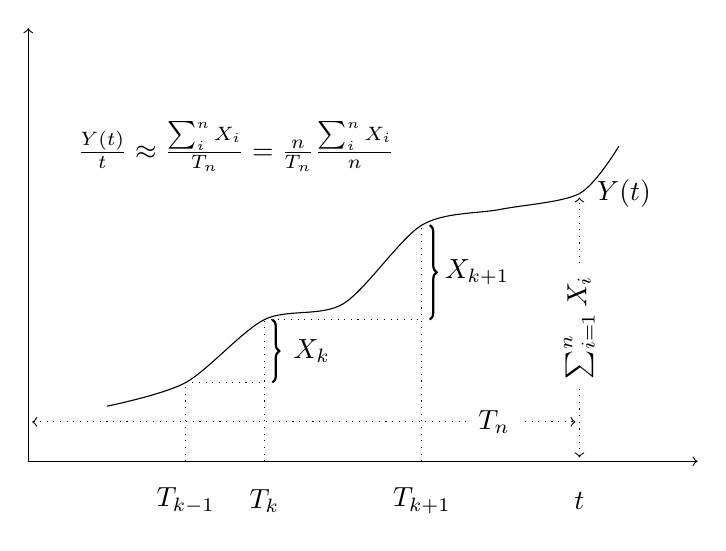
\begin{tikzpicture}[scale=1]
%axis
\draw[->] (0,0) -- coordinate (x axis mid) (8.5,0);
\draw[->] (0,0) -- coordinate (y axis mid) (0,5.5);
%\node[below=0.2cm] at (x axis mid) {$t$};

\draw plot [smooth] coordinates {(1,0.7) (2,1) (3,1.8) (4,2) (5,3) (6,3.2) (7, 3.4) (7.5,4.0)};
\node[right] at (7.1,3.4) {$Y(t)$};
\node at (7.,-0.5) {$t$};

\node at (2.,-0.5) {$T_{k-1}$};
\draw[dotted] (2,0)--(2,1);
\draw[dotted] (2,1)--(3,1);


\node at (3.,-0.5) {$T_{k}$};
\draw[dotted] (3,0)--(3,1.8);
\draw[dotted] (3,1.8)--(5,1.8);

\draw [
 thick,
 decoration={brace, mirror, raise=0.1cm },
 decorate
] (3,1) -- (3,1.8)
node[pos=0.5, xshift=0.6cm] {$X_k$};


\node at (5.,-0.5) {$T_{k+1}$};
\draw[dotted] (5,0)--(5,3);

\draw [
 thick,
 decoration={brace, mirror, raise=0.1cm },
 decorate
] (5,1.8) -- (5,3)
node[pos=0.5, xshift=0.7cm] {$X_{k+1}$};

\node[right] at (0.5,4) {$\frac{Y(t)}t \approx \frac{\sum_i^n X_i}{T_n} = \frac{n}{T_n} \frac{\sum_i^n X_i}n $};


\draw[dotted,<->, =stealth] (7,0.05)--(7,3.35) node[midway, rotate=90, fill=white] {$\sum_{i=1}^n X_i$};
\draw[dotted,<->, =stealth] (0.05,0.5)--(6.95,0.5) node[pos=0.85, fill=white] {$T_n$};
\end{tikzpicture}
\caption{A graphical `proof' of $Y=\lambda X$. }
\label{fig:renewal}
\end{figure}

\newthought{With the renewal reward theorem} we can relate the utilization $\rho=\lambda \E S$ to the limiting fraction of time the servers of a $G/G/c$ queue are busy.
In fact,  with this theorem\sidenote{~\cref{ex:l-162}}
\begin{equation}\label{eq:49}
 \lim_{t\to\infty} \frac 1 t \int_0^t \1{\L(s)>0} \d s = \delta \E S = \lambda \E S.
\end{equation}
Clearly, the LHS is the long-run fraction of time the servers are busy and RHS follows from rate-stability, i.e., $\delta=\lambda$.

We can derive\sidenote{\cref{ex:70}} this relation also by considering the fact that
\begin{equation}\label{eq:2a}
 \sum_{k=1}^{A(t)} S_k \geq \int_0^t \1{\L(s)>0} \d s \geq \sum_{k=1}^{D(t)} S_k.
\end{equation}
Then, by taking appropriate limits $\lambda \E S \geq \rho \geq \delta \E S$.
Rate-stability then completes the argument.


\begin{exercise}\label{ex:l-162}
Use the renewal reward theorem to prove \cref{eq:49}.
\begin{hint}
  Observe that $Y(t) = \int_0^t \1{\L(s)>0} \d s$ is the total amount of time the server has been busy up to the time $t$.
  Then take $T_k = D_k$ as the epochs at which to inspect $Y(t)$, and realize that $Y(D_{k}) = \sum_{i=1}^{k} S_{i}$.
  Use~\cref{eq:84}, i.e., rate stability.
\end{hint}
\begin{solution}
 It is evident that $X_k = Y(D_k)-Y(D_{k-1})=S_k$, hence $X = \lim_{n\to\infty} n^{-1}\sum_{k=1}^n X_k = \E S$.
% Also $\lim_{t\to\infty} Y(t)/t=\rho$.
 In the relation $Y = \lambda X$, the $\lambda$ is $\delta$ since we consider departure epochs $T_k = D_k$, rather than $A_k$.
 Thus, with the renewal reward theorem $Y=\lambda X$, we get that $Y = \lim_{t\to\infty} t^{-1} \int_0^t \1{\L(s)>0} \d s = \delta \E S$.
Observe that the $Y$ is the long-run fraction of time the server is busy.
\end{solution}
\end{exercise}


\begin{exercise}\label{ex:70}
Explain~\cref{eq:2a} and derive $\lambda \E S \geq \rho \geq \delta \E S$ from this.
\begin{hint}
For the direction of the inequalities~\cref{eq:2a}, observe that $t$ can lie half way a service interval, and $A(t) \geq D(t)$.
Divide by $t$ in~\cref{eq:2a}. Then for the LHS, multiply by $A(t)/A(t)$ and take appropriate limits. Similar for the RHS but multiply by $D(t)/D(t)$.
\end{hint}
\begin{solution}

  For the LHS, as $A(t)\to \infty$ as $t\to\infty$,
\begin{equation*}
 \lim_{t\to\infty} \frac 1 t\sum_{k=1}^{A(t)} S_k =
 \lim_{t\to\infty} \frac{A(t)}t \frac{1}{A(t)} \sum_{k=1}^{A(t)} S_k =
 \lim_{t\to\infty} \frac{A(t)}t \cdot \lim_{t\to\infty}\frac{1}{A(t)} \sum_{k=1}^{A(t)} S_k = \lambda \E S.
\end{equation*}
Apply similar limits to the RHS.
The limit of the middle term gives the fraction of time the server is busy.
\end{solution}
\end{exercise}



\opt{solutionfiles}{\Closesolutionfile{hint}
\Closesolutionfile{ans}
\loadgeometry{normal}
\input{hint}
\input{ans}
}

\end{document}


%%% Local Variables:
%%% mode: latex
%%% TeX-master: t
%%% End:
